\section{Durchführung}
\label{sec:Durchführung}
Die verwendet Messapparatur ist in \autoref{fig:messapparatur} dargestellt. Um Störspannungen zu vermeiden,
wird ein Selektivverstärker verwendet. Weiterhin werden zur Signalverstärkung 10xSignalverstärker verwendet.
\begin{figure}
    \centering
    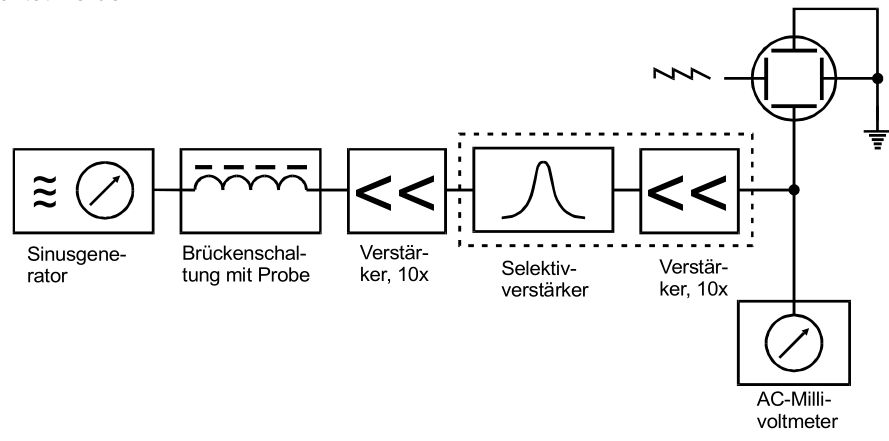
\includegraphics[width=0.7\textwidth]{bilder/messapparatur.png}
    \caption{Blockschaltbild der Messapparatur}
    \label{fig:messapparatur}
\end{figure}
Mit Hilfe eines Sinusgenerators können Frequenzen von $\SI{15}{\kilo\hertz}$ bis $\SI{40}{\kilo\hertz}$ erzeugt
werden. Um die Filterkurve zu bestimmen, wird an einem Voltmeter Messwerte im einstelligen Volt Bereich abgelesen
und die Frequenz in einem Bereich um das Spannungsmaximum eingestellt. Zur Bestimmung des Spannungsmaximus kann
aufgrund der einfacheren Ablesbarkeit ein Oszilloskop verwendet werden. Außerdem werden um das Spannungsmaximum
mehr Messwerte aufgenommen, da dort eine stärkere Steigung zu erwarten ist, die sich nur mit ausreichend
Messwerten gut darstellen lässt.

\subsection{Messung der Suszeptibilität}
\label{sec:messung}
Die Messwerte der zwei beschriebenen Verfahren zur Bestimmung der Suszeptibilität können der gleichen Messreihe
entnommen werden. Da die Proben im staubförmigen Material vorliegen, ist die Dichte der Proben geringer als
der eines Einkristalles. Die reale Querschnitt $Q_{\symup{Real}}$ bestimmt sich zu
\begin{equation}
    Q_{\symup{Real}} = Q\frac{M_{\symup{p}}}{l\rho_{\symup{w}}}\,.
\end{equation}
Dabei ist $M_{\symup{p}}$ die Masse, $l$ die Länge der Probe und $\rho_{w}$ die Dichte des Einkristalls. Die Länge
der Probe wird mit einer Schieblehre bestimmt. Weiterhin sollte die Probe nicht zu lange in der Hand gehalten
werden, da die Probe sich erwärmt und die Suszeptibilität temperaturabhägnig ist. Als erstes wird die durch den
variabel einstellbaren Widerstand $R_{\symup{P}}$ die Spannung auf ein Minimum geregelt und sowohl die gemessene
Spannung als auch der Widerstand werden aufgeschrieben. Danach wird die Probe eingeführt und die gemessene Spannung
notiert, um Messwerte für die erste Methode zu erhalten. Weiterhin wird die Spannung erneut über den regelbaren
Widerstand minimiert und aufgeschrieben, so dass sich auch Messwerte für die zweite Methode zu Bestimmung der
Suszeptibilität ergeben. Dieses Verfahren wird für drei unterschiedliche Proben seltener Erden je dreimal
wiederholt.